\clearpage
\section{Norton Guide: \RU{простейшее однобайтное XOR-шифрование}\EN{simplest possible 1-byte XOR encryption}}

\EN{Norton Guide\footnote{\href{http://go.yurichev.com/17116}{wikipedia}} was popular in the epoch of MS-DOS, it was a resident program that worked as a hypertext reference manual.}
\RU{Norton Guide\footnote{\href{http://go.yurichev.com/17116}{wikipedia}} был популярен во времена MS-DOS, это была резидентная программа, работающая как
гипертекстовый справочник.}

\EN{Norton Guide's databases are files with the extension .ng, the contents of which look encrypted:}
\RU{Базы данных Norton Guide это файлы с расширением .ng, содержимое которых выглядит как зашифрованное:}

\begin{figure}[H]
\centering
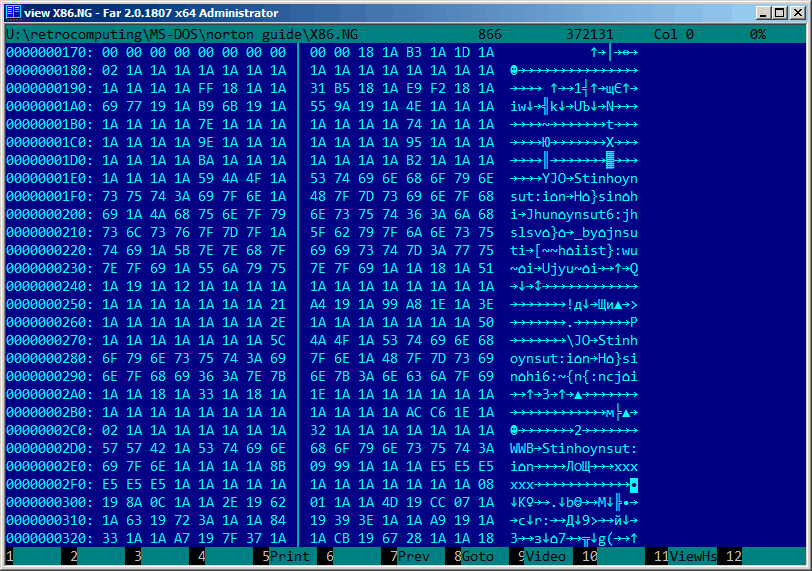
\includegraphics[scale=\FigScale]{ff/XOR/ng/ng1.png}
\caption{\RU{Очень типичный вид}\EN{Very typical look}}
\end{figure}

\EN{Why did we think that it's encrypted but not compressed?}%
\RU{Почему мы думаем, что зашифрованное а не сжатое? }
\EN{We see that the 0x1A byte (looking like \q{$\rightarrow$}) occurs often, it would not be possible in a compressed file.}
\RU{Мы видим, как слишком часто попадается байт 0x1A (который выглядит как \q{$\rightarrow$}), в сжатом файле такого не было бы никогда.}
\EN{We also see long parts that consist only of latin letters, and they look like strings in an unknown
language.}
\RU{Во-вторых, мы видим длинные части состоящие только из латинских букв, они выглядят как строки
на незнакомом языке.}

\clearpage
\EN{Since the 0x1A byte occurs so often, we can try to decrypt the file, assuming that it's encrypted
by the simplest XOR-encryption.}
\RU{Из-за того, что байт 0x1A слишком часто встречается, мы можем попробовать расшифровать файл, полагая
что он зашифрован простейшим XOR-шифрованием.}
\EN{If we apply XOR with the 0x1A constant to each byte in Hiew, we can see familiar English text strings:}
\RU{Применяем XOR с константой 0x1A к каждому байту в Hiew и мы можем видеть знакомые текстовые строки на английском:}

\begin{figure}[H]
\centering
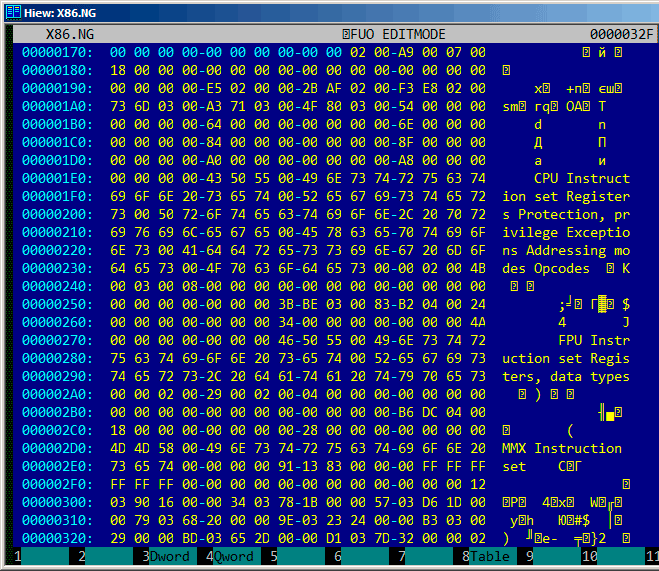
\includegraphics[scale=\FigScale]{ff/XOR/ng/ng2.png}
\caption{Hiew \RU{применение XOR с 0x1A}\EN{XORing with 0x1A}}
\end{figure}

\EN{XOR encryption with one single constant byte is the simplest possible encryption method, which is, nevertheless,
encountered sometimes.}
\RU{XOR-шифрование с одним константным байтом это самый простой способ шифрования, который, тем не менее, иногда
встречается.}

\EN{Now we understand why the 0x1A byte was occurring so often: because there are so many zero bytes and they
were replaced by 0x1A in encrypted form.}
\RU{Теперь понятно почему байт 0x1A так часто встречался: потому что в файле очень много нулевых байт 
и в зашифрованном виде они везде были заменены на 0x1A.}

\EN{But the constant might be different}\RU{Но эта константа могла быть другой}.
\EN{In this case, we could try every constant in the 0..255 range and look for something familiar in the decrypted
file. 256 is not so much.}
\RU{В таком случае, можно было бы попробовать перебрать все 256 комбинаций, и посмотреть содержимое \q{на глаз}, 
а 256 --- это совсем немного.}

\EN{More about Norton Guide's file format:}
\RU{Больше о формате файлов Norton Guide:} \url{http://go.yurichev.com/17317}.

\subsection{\RU{Энтропия}\EN{Entropy}}
\index{Wolfram Mathematica}
\index{\RU{Энтропия}\EN{Entropy}}

\EN{A very important property of such primitive encryption systems is that the information entropy
of the encrypted/decrypted block is the same.}
\RU{Очень важное свойство подобного примитивного шифрования в том, что информационная энтропия
зашифрованного/дешифрованного блока точно такая же.}
\EN{Here is my analysis in}\RU{Вот мой анализ в} Wolfram Mathematica 10.

\begin{lstlisting}[caption=Wolfram Mathematica 10]
In[1]:= input = BinaryReadList["X86.NG"];

In[2]:= Entropy[2, input] // N
Out[2]= 5.62724

In[3]:= decrypted = Map[BitXor[#, 16^^1A] &, input];

In[4]:= Export["X86_decrypted.NG", decrypted, "Binary"];

In[5]:= Entropy[2, decrypted] // N
Out[5]= 5.62724

In[6]:= Entropy[2, ExampleData[{"Text", "ShakespearesSonnets"}]] // N
Out[6]= 4.42366
\end{lstlisting}

\EN{What we do here is load the file, get its entropy, decrypt it, save it and get the entropy again (the same!).}
\RU{Что мы здесь делаем это загружаем файл, вычисляем его энтропию, дешифруем его, сохраняем, снова вычисляем энтропию (точно такая же!).}
\EN{Mathematica also offers some well-known English language texts for analysis.}
\RU{Mathematica дает возможность анализировать некоторые хорошо известные англоязычные тексты.}
\EN{So we also get the entropy of Shakespeare's sonnets, and it is close to the entropy of the file we just analyzed.}
\RU{Так что мы вычисляем энтропию соннетов Шейкспира, и она близка к энтропии анализируемого нами файла.}
\EN{The file we analyzed consists of English language sentences, which are close to the language 
of Shakespeare.}
\RU{Анализируемый нами файл состоит из предложений на английском языке, которые близки к языку
Шейкспира.}
\EN{And the XOR-ed bitwise English language text has the same entropy.}
\RU{И применение побайтового XOR к тексту на английском языке не меняет энтропию.}

% I checked!
\EN{However, this is not true when the file is XOR-ed with a pattern larger than one byte.}
\RU{Хотя, это не будет справедливо когда файл зашифрован при помощи XOR 
шаблоном длинее одного байта.}

\EN{The file we analyzed can be downloaded here}\RU{Файл, который мы анализировали, 
можно скачать здесь}: \url{http://go.yurichev.com/17350}.

\subsubsection{\EN{One more word about base of entropy}\RU{Еще кое-что о базе энтропии}}

\newcommand{\FNENTURL}{\footnote{\url{http://www.fourmilab.ch/random/}}}

\EN{Wolfram Mathematica calculates entropy with base of $e$ (base of the natural logarithm),
and the UNIX \IT{ent} utility\FNENTURL uses base 2.}
\RU{Wolfram Mathematica вычисляет энтропию с базой $e$ (основание натурального логарифма),
а утилита UNIX \IT{ent}\FNENTURL использует базу 2.}
\EN{So we set base 2 explicitly in \TT{Entropy} command, so Mathematica will give us the same results as the \IT{ent} utility.}
\RU{Так что мы явно указываем базу 2 в команде \TT{Entropy}, чтобы Mathematica давала те же результаты, что и утилита \IT{ent}.}
